\documentclass[a4paper,12pt]{article}
\usepackage{color}
\usepackage{amsmath} % do fancy math
\usepackage{mathtools}
\usepackage{amsfonts}
\usepackage{bm}
\usepackage{amsthm} % math theorem proof etc
\usepackage{graphicx} % import images
\usepackage{tikz} % draw images with latex
%\usetikzlibrary{arrows,decorations.pathmorphing,backgrounds,positioning,fit,petri}
\usepackage{pgf} % go with tikz
\usepackage{subfigure}
\usepackage{caption}
%\usepackage{subcaption}
\usepackage{multirow}
\usepackage{algorithm}
\usepackage{algorithmic}
\usepackage{epstopdf}
\usepackage[round]{natbib}
\usepackage{setspace}
\usepackage[top=30mm, bottom=30mm, left=35mm,right=30mm]{geometry}
\newcommand{\ud}{\,\mathrm{d}}
\newcommand{\vx}{\mathbf{x}}
\newtheorem{defi}{Definition}[section]
\newtheorem{theorem}{Theorem}[section]
\newtheorem{lemma}[theorem]{Lemma}
%------------Y(^_^) I'm the happy separation line (^_^)Y-------------%


%------------Y(^_^) I'm the toolbox for lazybones (^_^)Y-------------%
% Maths
% \begin{equation*}
%
% \end{equation*}
% \mathcal{}
% \!  \,  \:  \;

% Graph
% \begin{figure}[htbp]
% \begin{center}
% \includegraphics[scale=1.1,trim=2cm 0cm 0cm 2cm]{name.pdf}
% \end{center}
% \caption[short]{long}
% \label{fig:3.2}
% \end{figure}

% Fonts
% \textbf{} \textsf{} \textit{} \textt{}

% Paragraph
% \onehalfspacing  \doublespacing
% setlength{\parindent}{0in}

% title
% \title{}
% \author{Zhe Sha}
% \date{1-Jan-1111}
% \maketitle

%------------Y(^_^) I'm the toolbox for lazybones (^_^)Y-------------%
\begin{document}

\title{Experiment 1a}
\author{Zhe Sha}
\maketitle

\onehalfspacing
\numberwithin{equation}{section}
%------------Y(^_^) I'm the happy separation line (^_^)Y-------------%

\section{Introduction}
In this report we present results of Experiment 1a that focuses on updating a uni-variate process with single source of observations. The main purpose is to develop a complete implementation of the Bayesian hierarchical model framework on the sphere that is simple enough for debugging and tuning (model or algorithm related) parameters.

In Experiment 1a, we test on the GIA process with synthetic GPS data. Over the period of 2005 to 2015, we assume the GIA process is a time invariant spatial process that represent a yearly trend in $mm$. The GPS data are processed to reflect only the vertical movement of the earth, also in $mm/yr$. Denote the GIA process by $X_{GIA}$ and the GPS observation by $Y_{GPS}$, then the Bayesian hierarchical model can be written as
\begin{align}
\left\{\begin{array}{l}
\bm{Y}_{GPS} | \bm{X}_{GIA}, \bm{e} = \bm{A} \bm{X}_{GIA} + \bm{e} \\
\bm{X}_{GIA} | \bm{\mu}_{GIA}, \bm{Z}_{GIA} = \bm{\mu}_{GIA} + \bm{Z}_{GIA} \\
\bm{Z}_{GIA} | \rho, \sigma^2 \sim \mathcal{GP}(0, K_{\nu}(\cdot, \cdot \, | \rho, \sigma^2)),  \; \bm{e} \sim \mathcal{N} (0, \sigma_e^2 \bm{I})
\end{array}
\right.
\end{align} 
where $A$ is the linear mapping operator from the process to the observations, $\bm{e}$ is a vector of the measurement errors of the GPS data, $\bm{\mu}_{GIA}$ is the prior GIA mean field which can usually be derived from some physical models, $\bm{Z}_{GIA}$ is a stationary zero mean Gaussian spatial process with Mat\'{e}rn covariance function, and $\rho, \sigma^2, \sigma_e^2$ are the hyper-parameters to be estimated.   

In the following, we use the ICE-6G results on one degree resolution as the prior GIA mean field. The synthetic data are generated by adding Gaussian noises to the ICE-6G data at the location of the selected GPS station. 



\section{Priors for the hyper parameters }
2. Transformation of the hyper parameter and choosing the prior

\newpage
\section{Test error size}
3. Test the "Principle of stable inference" theorem 
\subsection{Change error size of a single point}
 Compare the effect of error size using a single isolated point.
 
 \begin{figure}[htbp]
 \begin{center}
 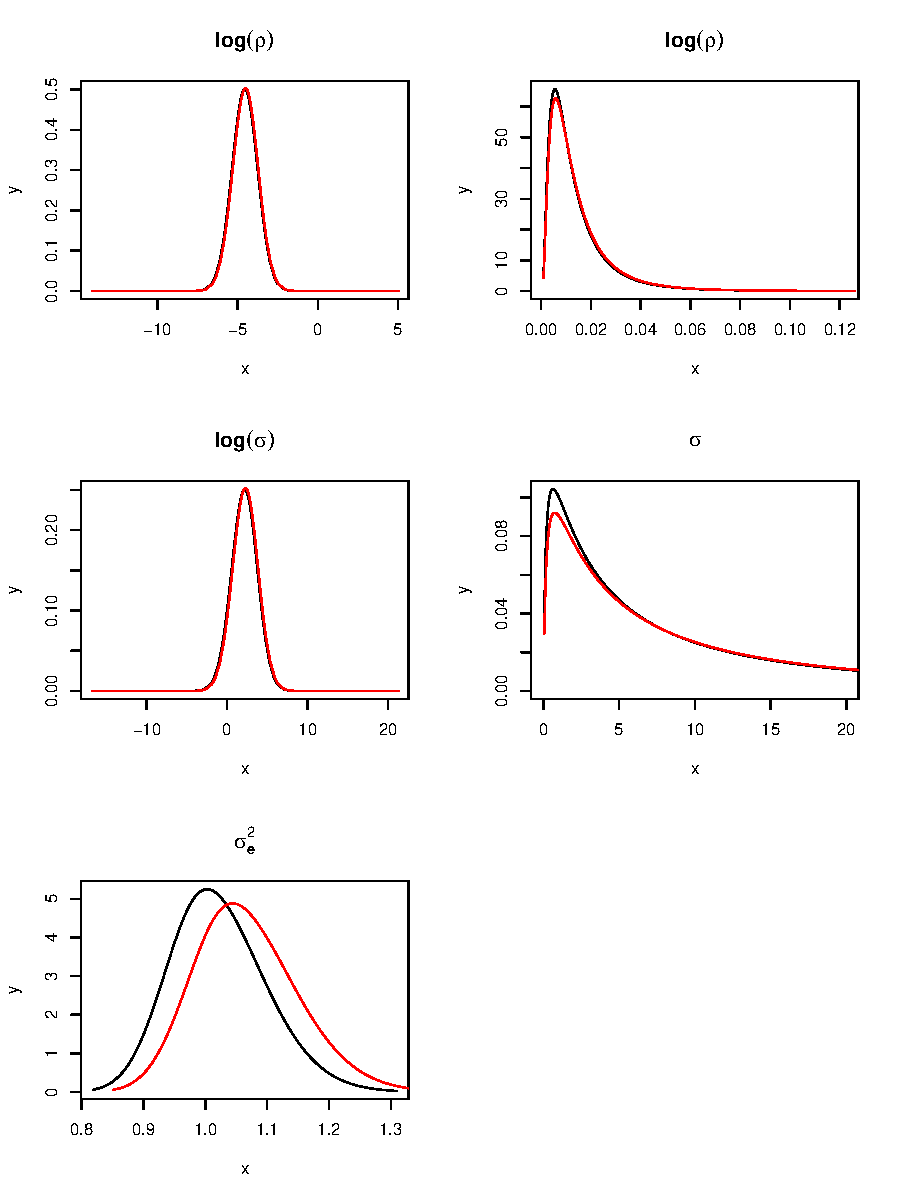
\includegraphics[scale=0.8]{fig/PointErr_hyperpar.pdf}
 \end{center}
 \caption[Posteriors of hyper parameters]{Posteriors of the hyper parameters using different error size for a selected point. Black: small error, Red: large error.}
 \label{fig:5}
 \end{figure}
 
 \begin{figure}[htbp]
 \begin{center}
 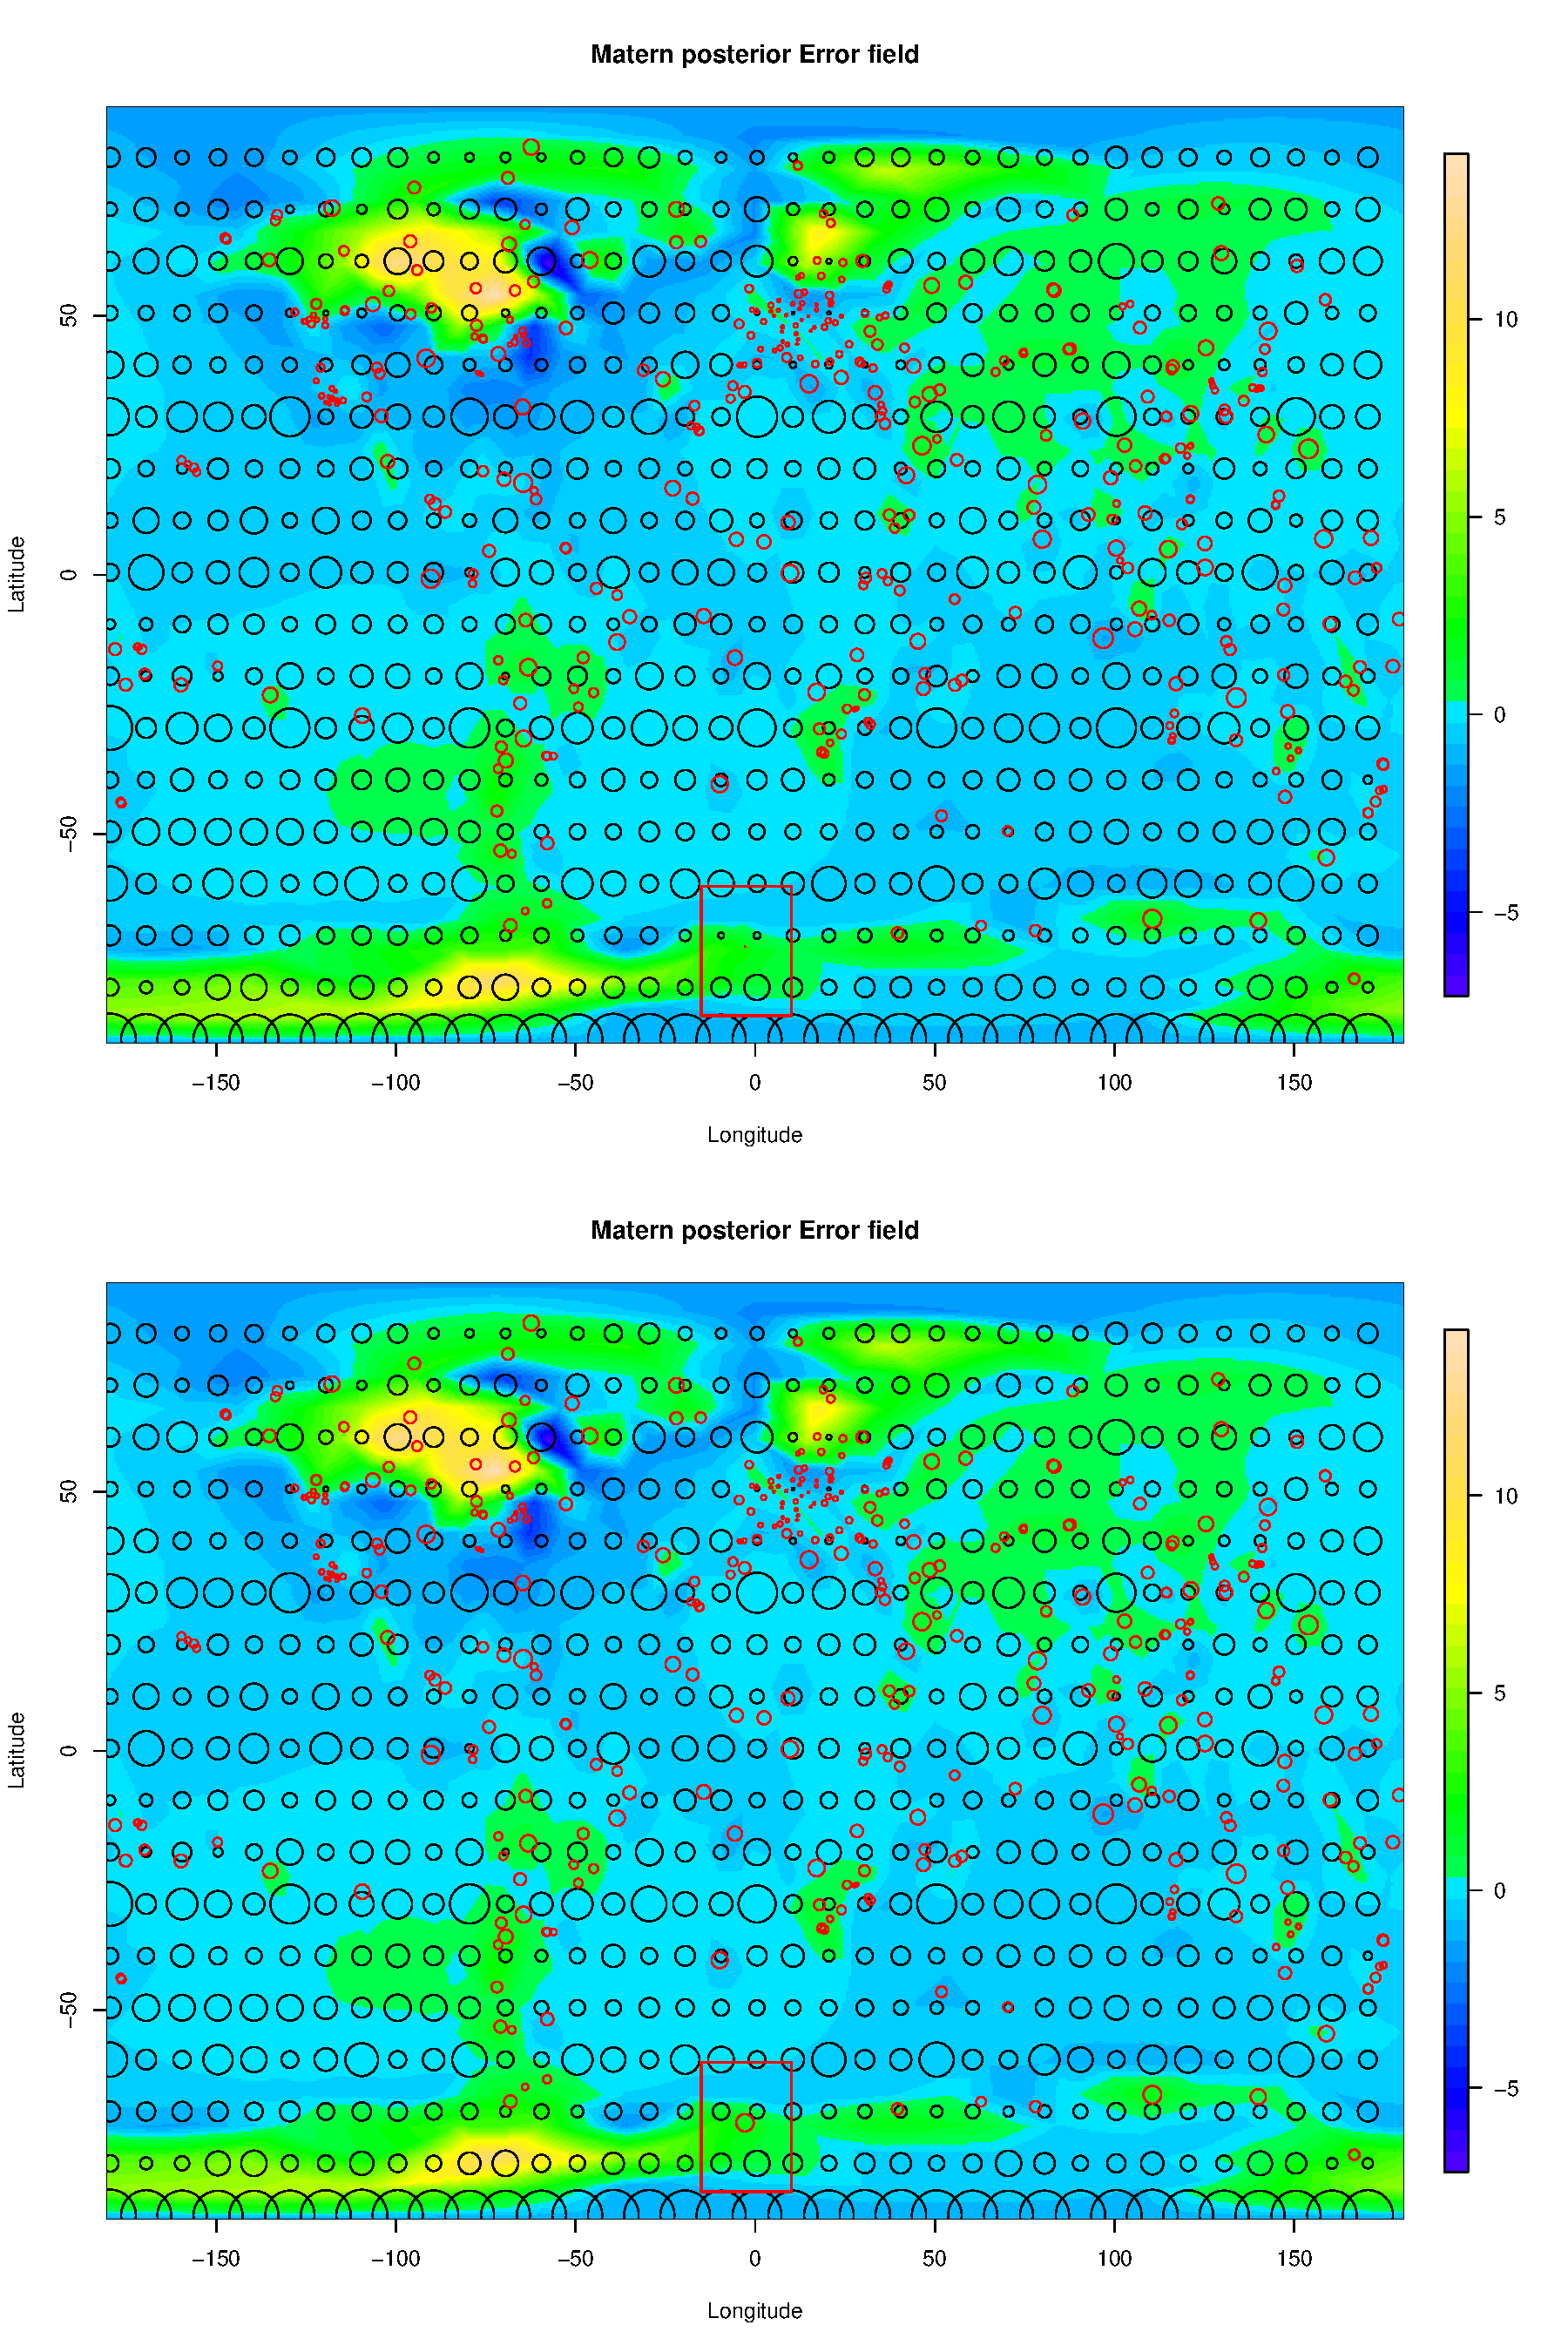
\includegraphics[scale=0.8]{fig/PointErr_GIAfield.pdf}
 \end{center}
 \caption[Posterior marginal standard errors of the latent field]{Posteriors marginal standard errors of the latent field using GPS data with different error on a single selected point. The selected point is marked as the circle within the red rectangle. Points are the GPS locations. Red points are positive errors and black negative. The circle size in the bottom plot represents the error size.}
 \label{fig:6}
 \end{figure}
 
 \newpage
 \subsection{Change global error size}

 \begin{figure}[htbp]
 \begin{center}
 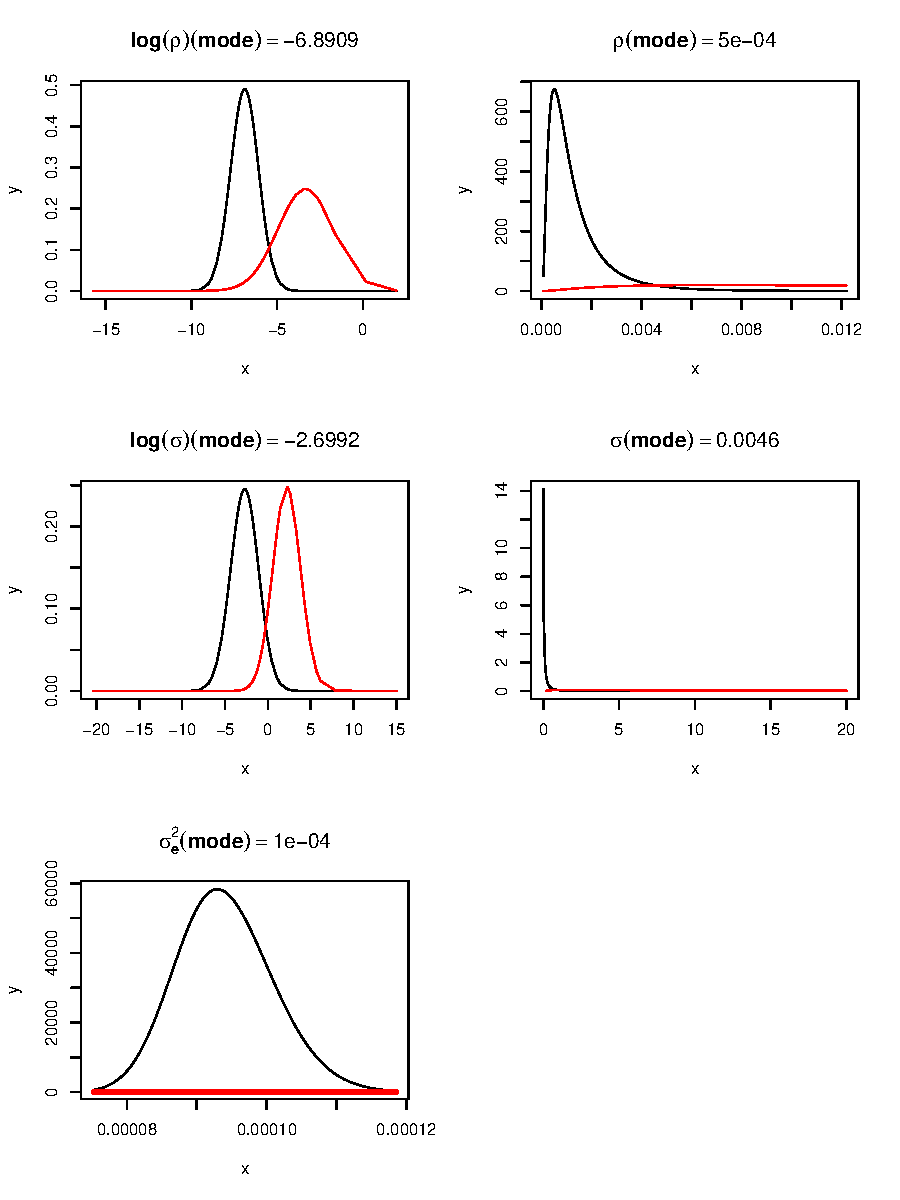
\includegraphics[scale = 0.8]{fig/sMesh_sErr_hyperpar.pdf}
 \end{center}
 \caption[Hyper parameter with small errors]{Posteriors of hyper parameters using GPS data with small measurement errors. Black: posterior, Red: prior.}
 \label{fig:1}
 \end{figure}

\begin{figure}[htbp]
 \begin{center}
 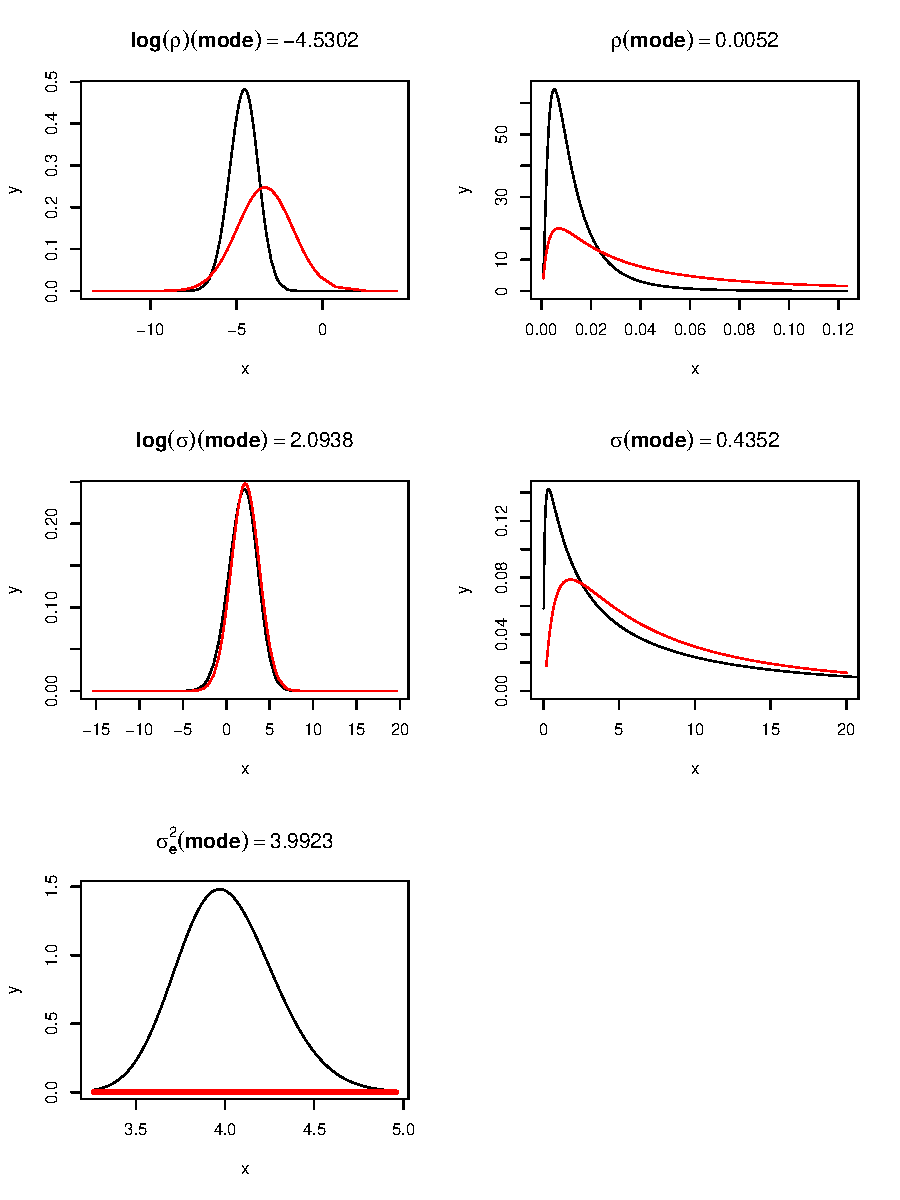
\includegraphics[scale = 0.8]{fig/sMesh_LErr_hyperpar.pdf}
 \end{center}
 \caption[Hyper parameter with large errors]{Posteriors of hyper parameters using GPS data with large measurement errors. Black: posterior, Red: prior.}
 \label{fig:2}
 \end{figure}
 
  \begin{figure}[htbp]
 \begin{center}
 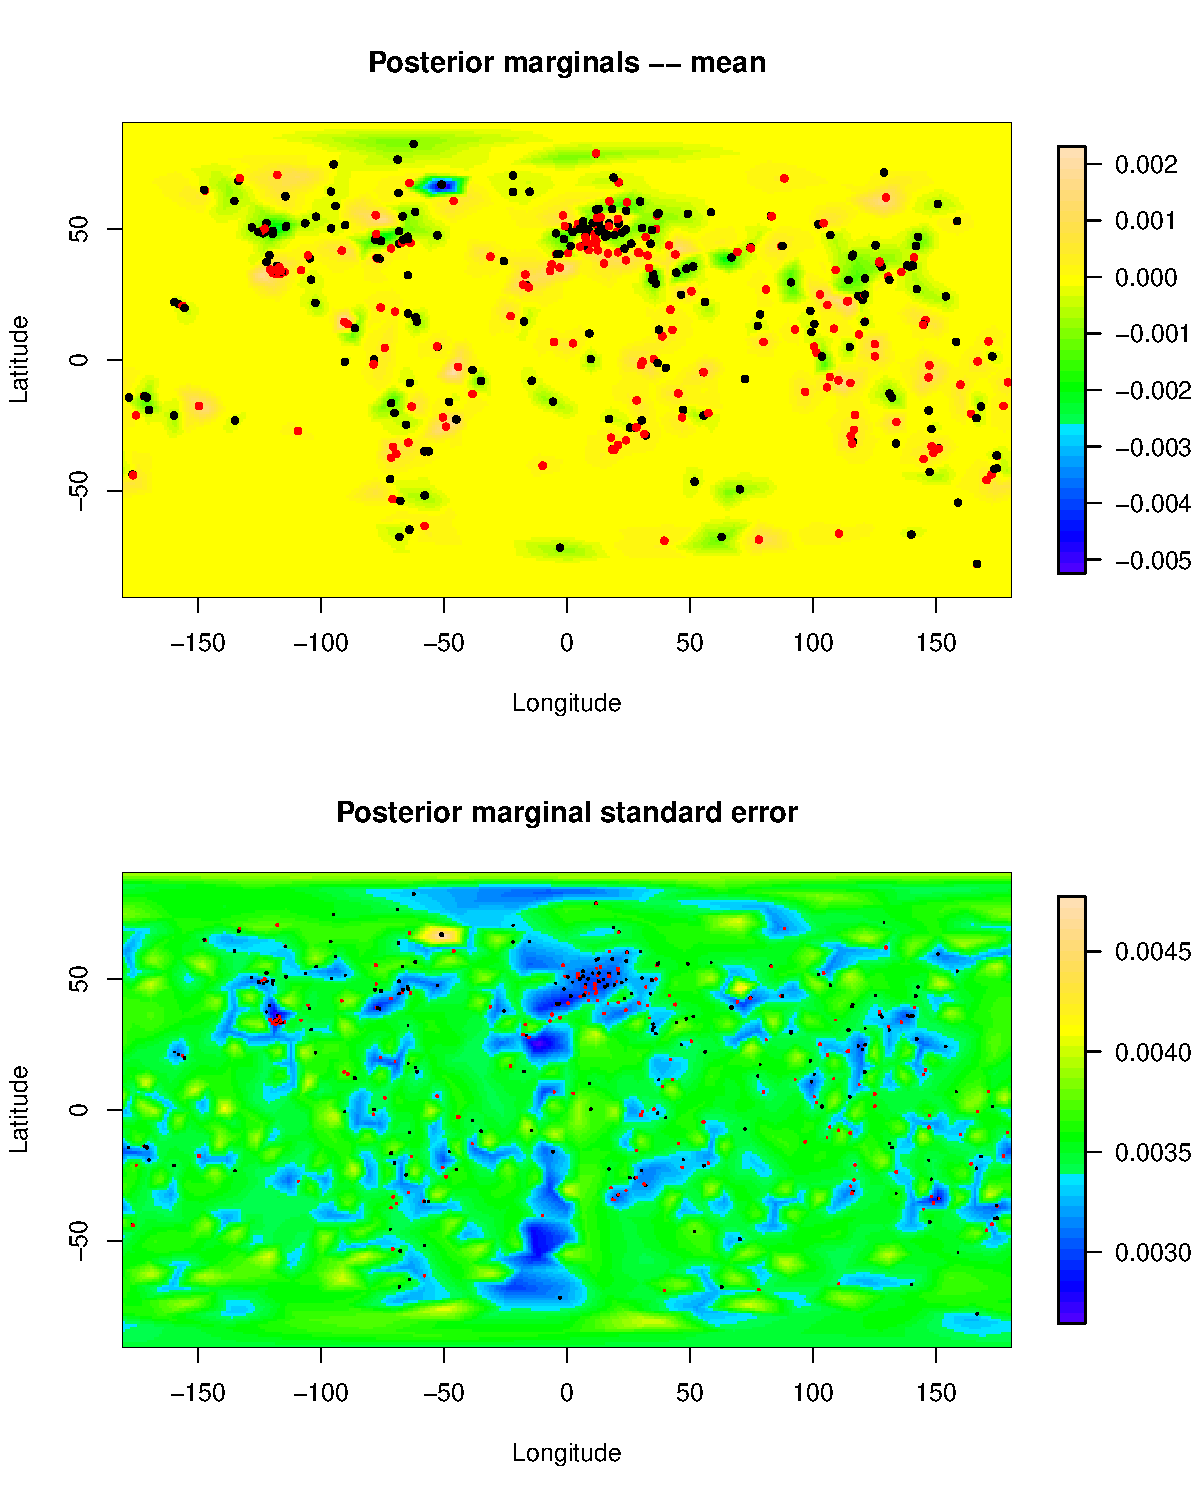
\includegraphics[scale=0.8]{fig/sMesh_sErr_GIAfield.pdf}
 \end{center}
 \caption[Posterior marginals of the latent field]{Posteriors marginal means and standard errors of the latent field using GPS data with small measurement errors. Points are the GPS locations. Red points are positive errors and black negative. The circle size in the bottom plot represents the error size.}
 \label{fig:3}
 \end{figure}
 
 \begin{figure}[htbp]
 \begin{center}
 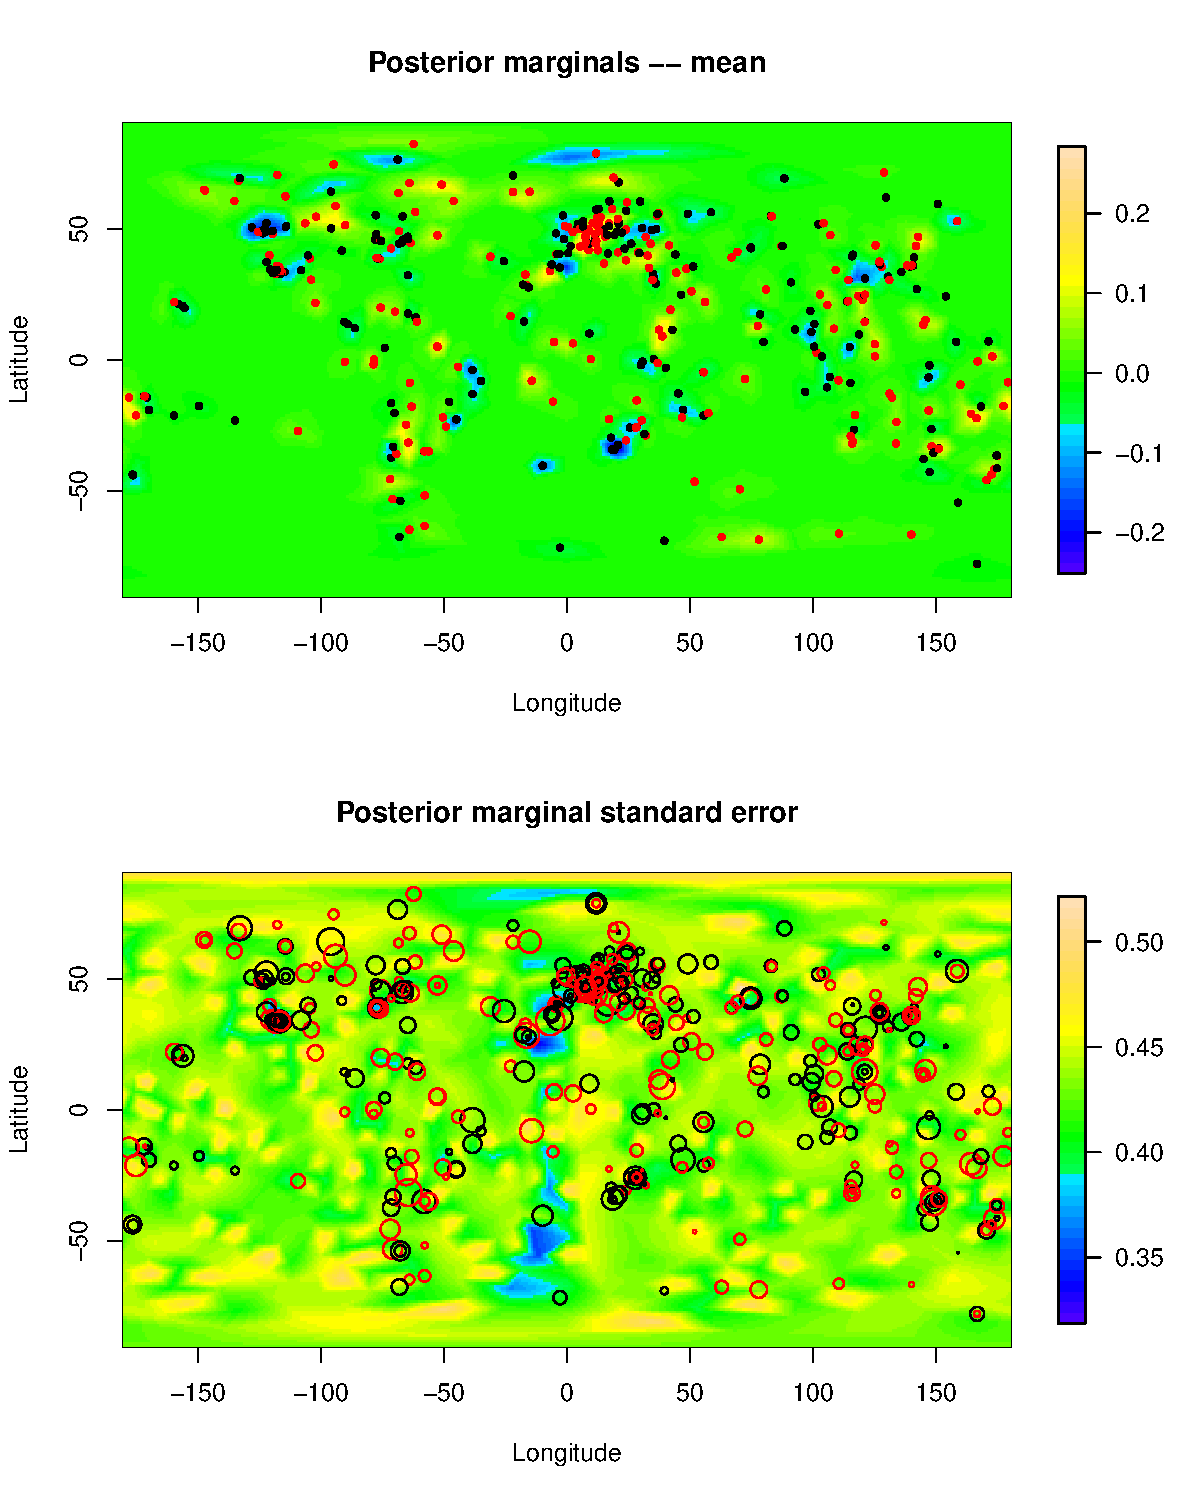
\includegraphics[scale=0.8]{fig/sMesh_LErr_GIAfield.pdf}
 \end{center}
 \caption[Posterior marginals of the latent field]{Posteriors marginal means and standard errors of the latent field using GPS data with large measurement errors. Points are the GPS locations. Red points are positive errors and black negative. The circle size in the bottom plot represents the error size.}
 \label{fig:4}
 \end{figure}
 
 \newpage
 
\section{Effect of Mesh size}

\begin{figure}[htbp]
 \begin{center}
 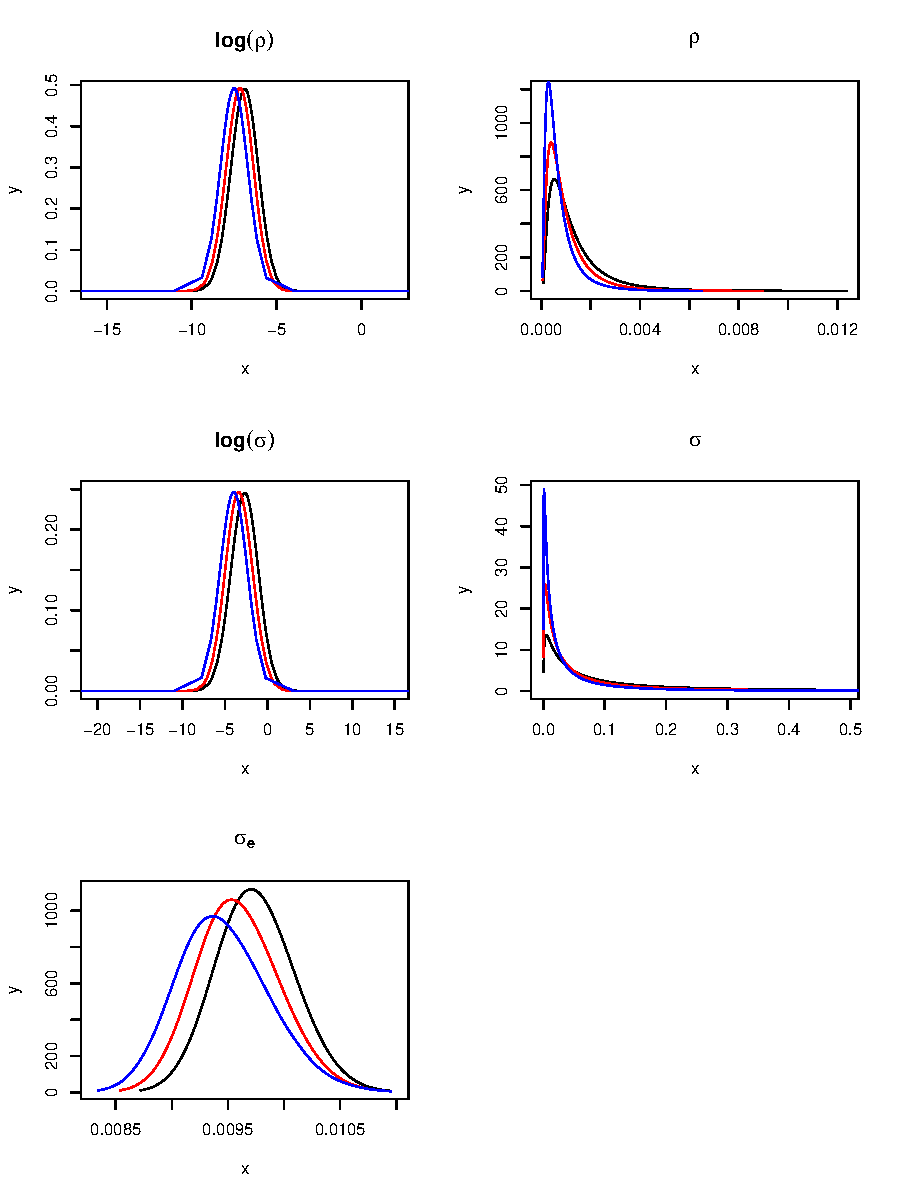
\includegraphics[scale = 0.8]{fig/MeshSize_1hyperpar.pdf}
 \end{center}
 \caption[Hyper parameter for different mesh sizes]{Posteriors of hyper parameters estimated using different mesh sizes for the latnet process. Black: small, Red: medium, blue: large.}
 \label{fig:2}
 \end{figure}


 \begin{figure}[htbp]
 \begin{center}
 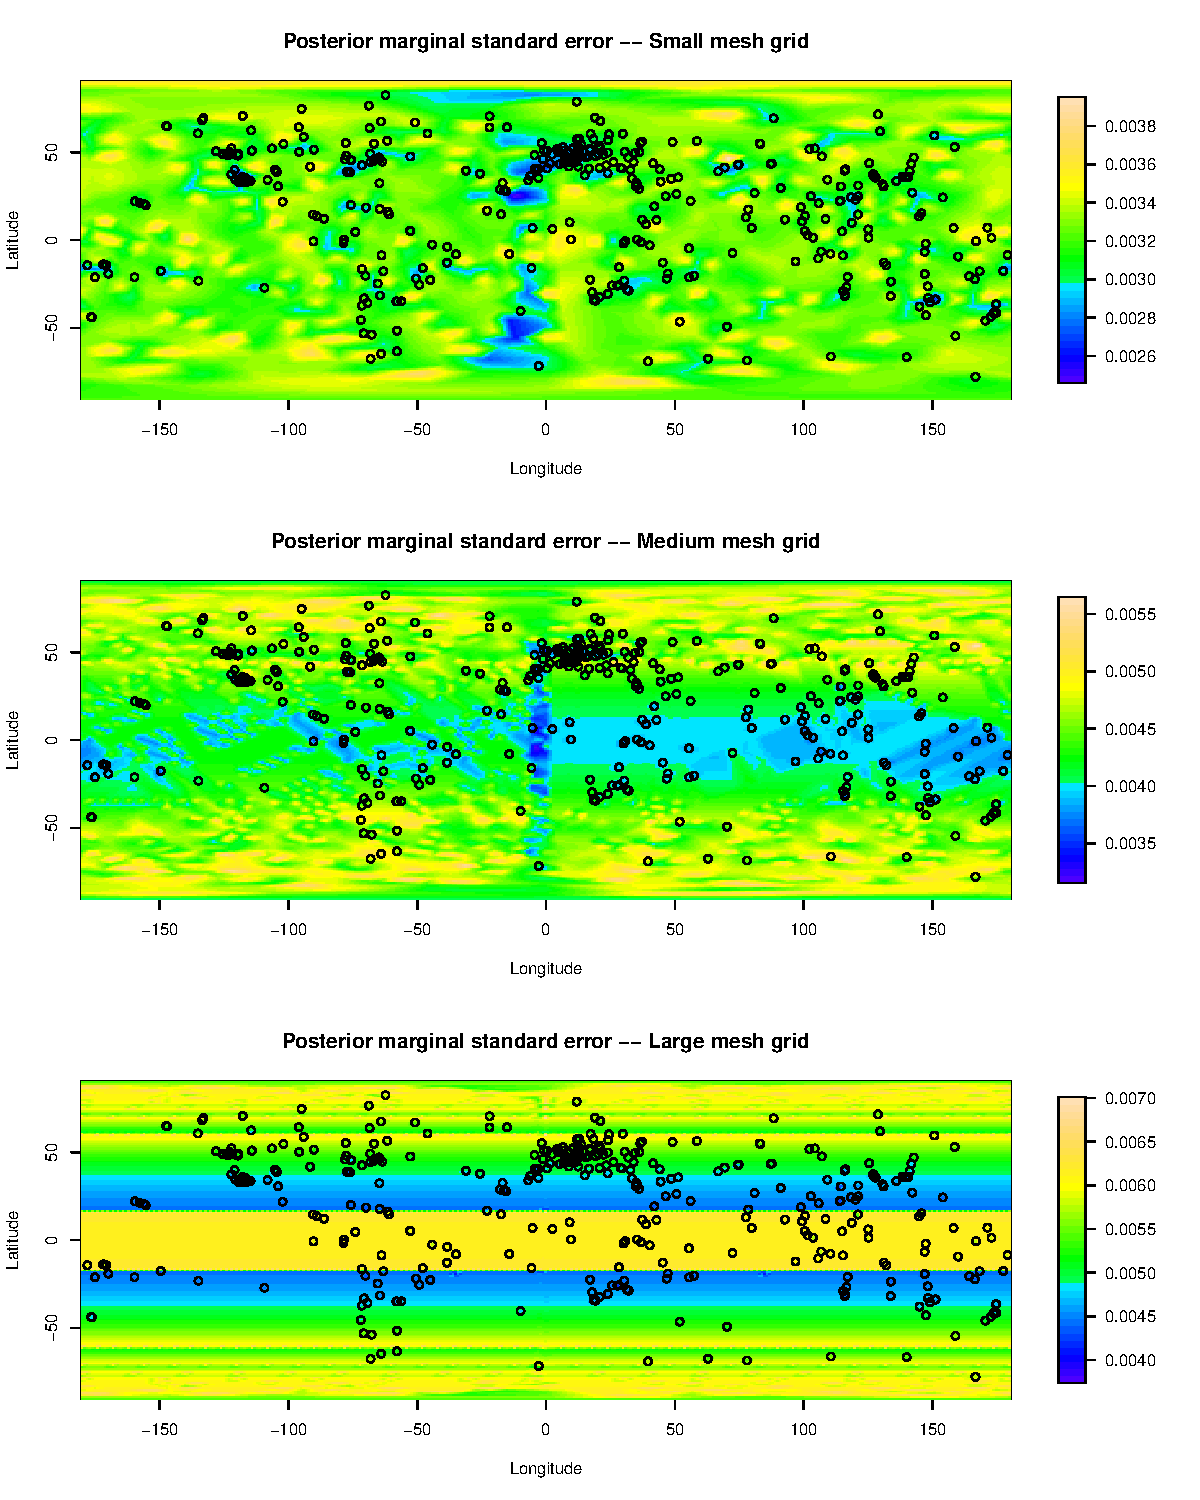
\includegraphics[scale=0.8]{fig/MeshSize_1GIAfield.pdf}
 \end{center}
 \caption[Posterior marginals of the latent field from different mesh size]{Posteriors marginal standard errors of the latent field with different mesh sizes. Points are the GPS locations.}
 \label{fig:4}
 \end{figure}
 

\section{MCMC results}

All tested on the smallest mesh grid and use univariate slice sampler for updating the SPDE parameters.





\section{Experiment 1b}


\begin{figure}[htbp]
 \begin{center}
 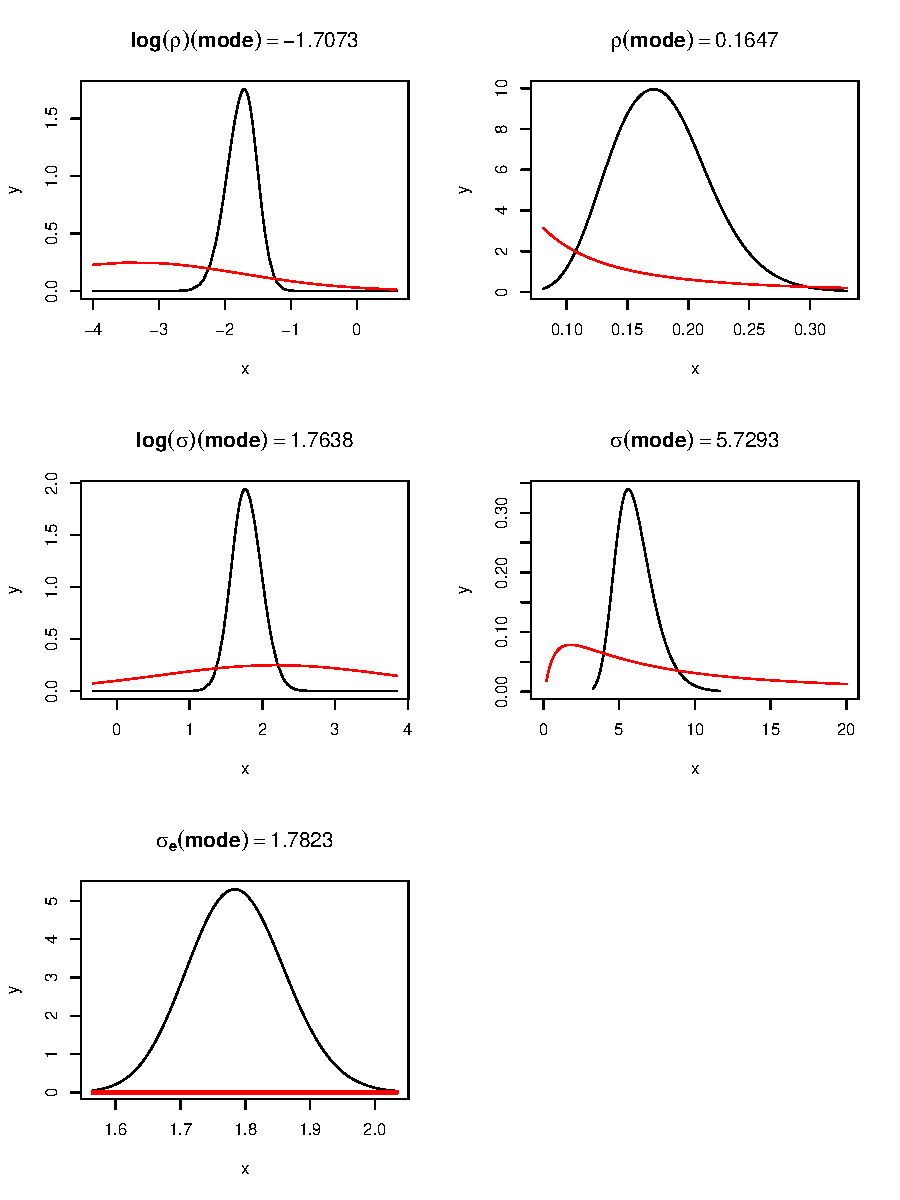
\includegraphics[scale=0.8]{fig/1bsMesh_hyperpar.pdf}
 \end{center}
 \caption[Posterior hyper parameters]{Posteriors of the hyper parameters using INLA.}
 \label{fig:5}
 \end{figure}


\begin{figure}[htbp]
 \begin{center}
 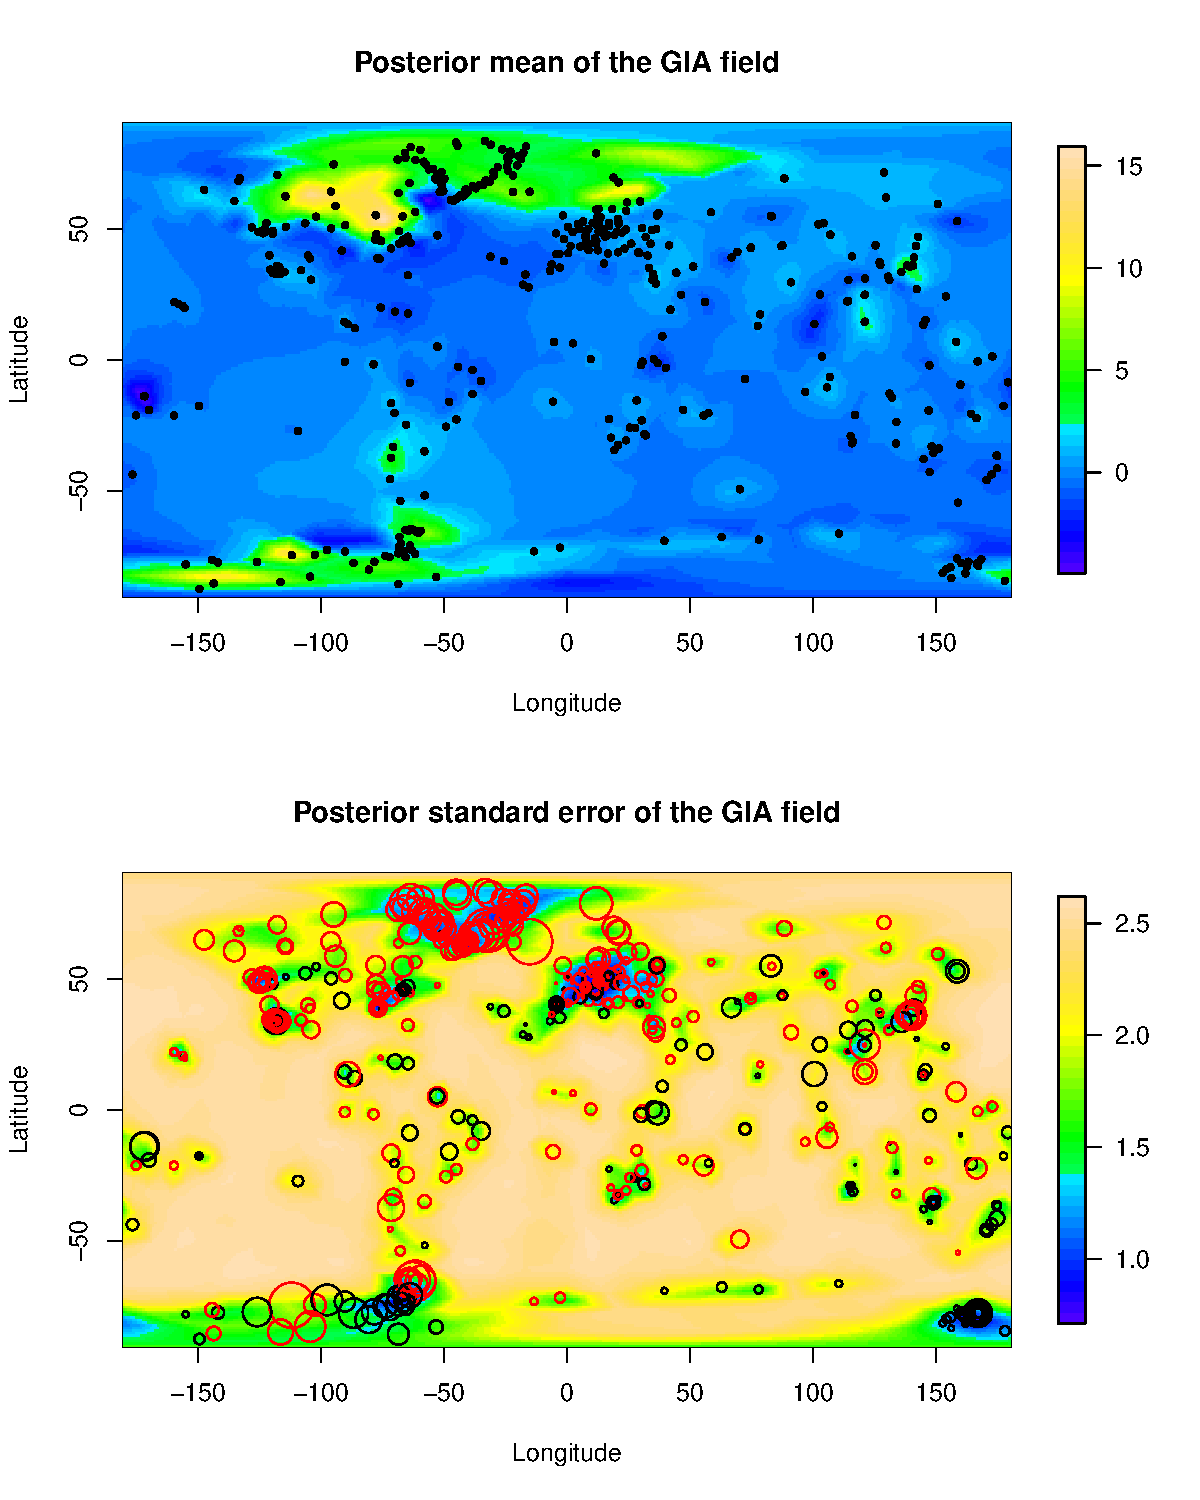
\includegraphics[scale=0.8]{fig/1bsMesh_GIAfield.pdf}
 \end{center}
 \caption[Posterior field]{Posteriors GIA field using INLA.}
 \label{fig:5}
 \end{figure}
 
 \begin{figure}[htbp]
 \begin{center}
 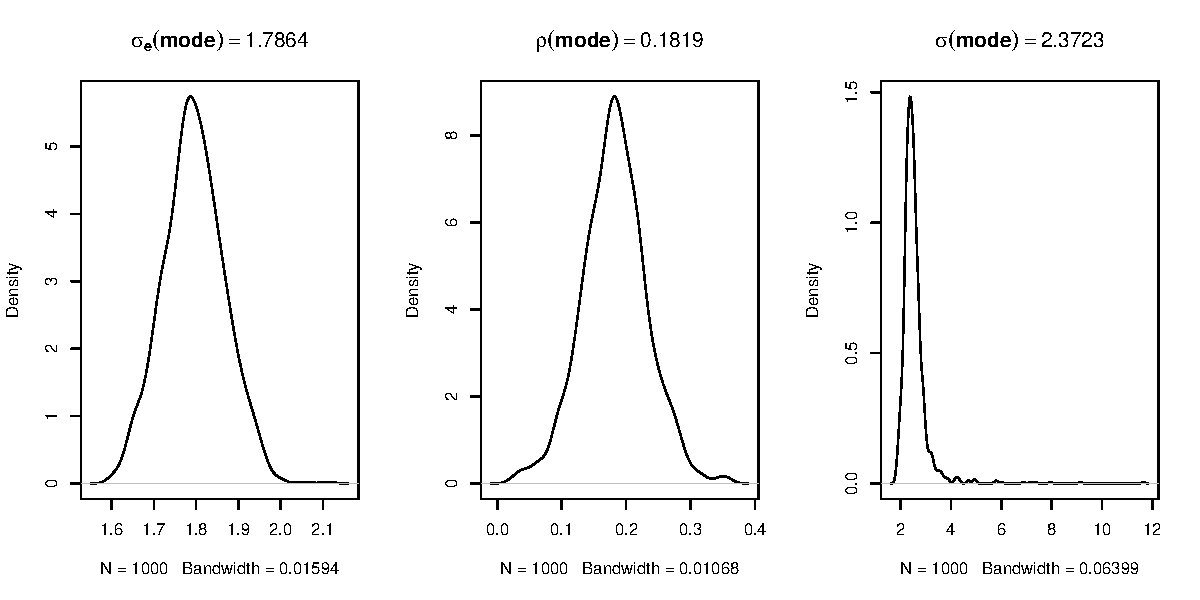
\includegraphics[scale=0.8]{fig/1bslice1_1000_hyperpars.pdf}
 \end{center}
 \caption[Posterior hyper parameters]{Posteriors of the hyper parameters using MCMC.}
 \label{fig:5}
 \end{figure}
 
 \begin{figure}[htbp]
 \begin{center}
 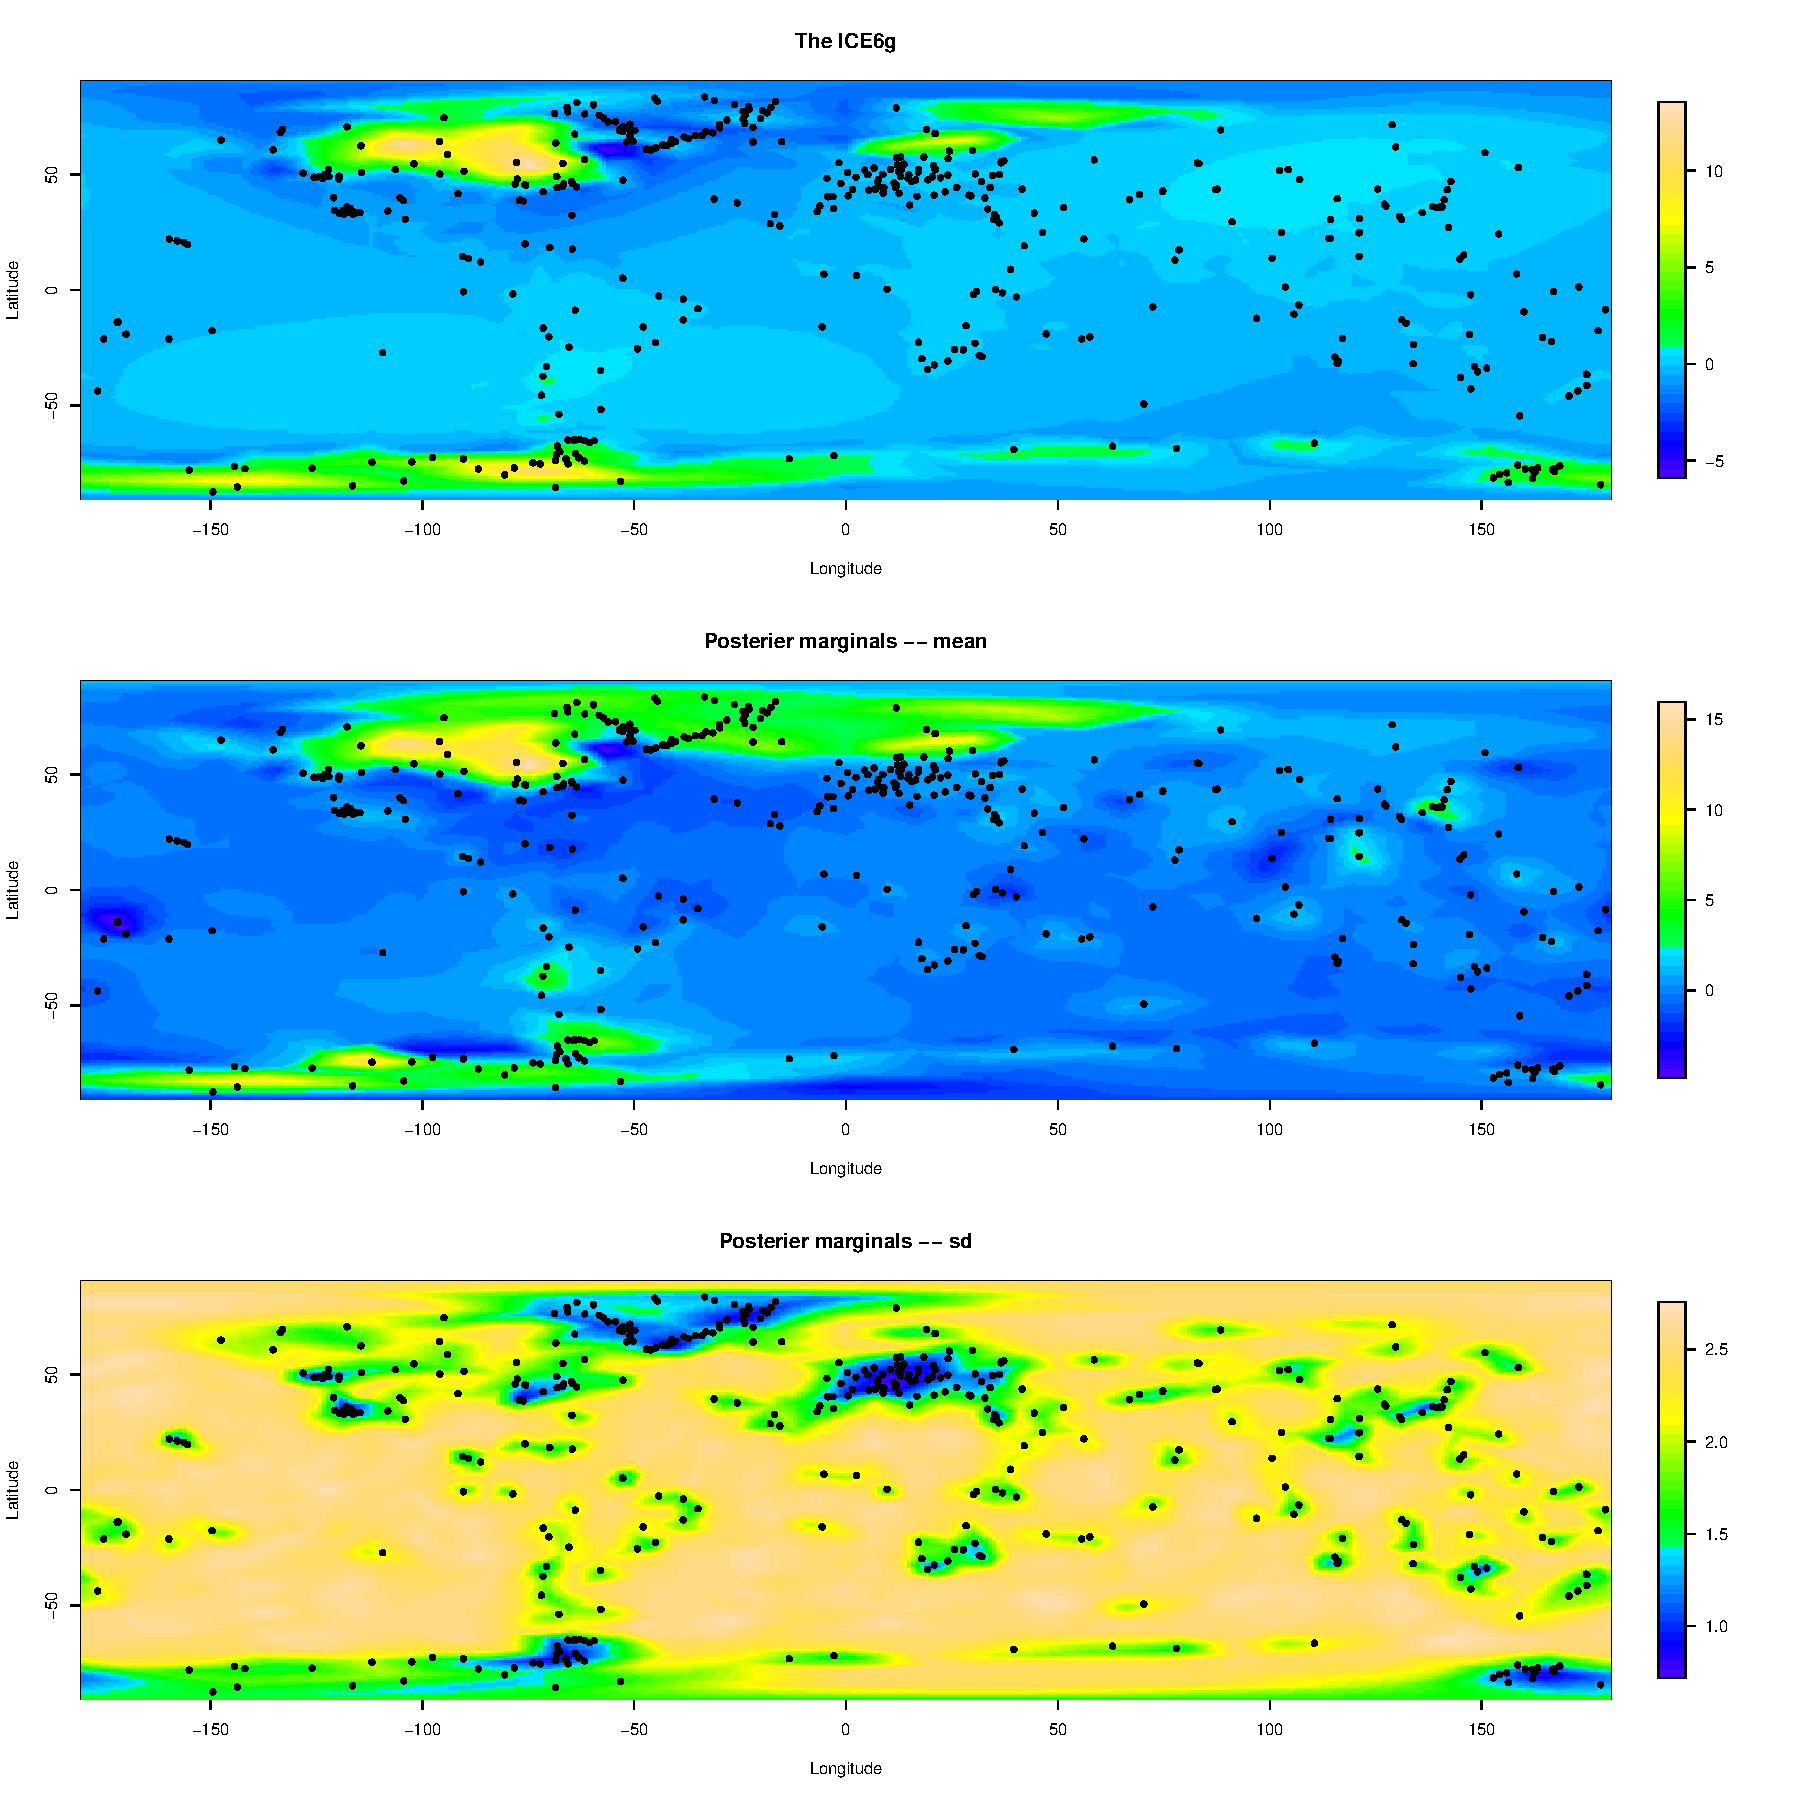
\includegraphics[scale=0.55]{fig/1bslice1_1000_GIAfield1.pdf}
 \end{center}
 \caption[Posterior field]{Posteriors GIA field using MCMC.}
 \label{fig:5}
 \end{figure}
 
 
 

%------------Y(^_^) I'm the happy separation line (^_^)Y-------------%
\bibliographystyle{abbrvnat}
%\bibliography{references}




\end{document}